\documentclass{article}
\usepackage[margin=2.54cm]{geometry}
\usepackage{graphicx}   % imágenes
\graphicspath{{img}}
\usepackage{amsfonts}   % fuentes de conjuntos numéricos
\usepackage{amsmath}
\usepackage{tikz}       % gráficos
\usepackage{pgfplots}   % plots
\pgfplotsset{width=10cm, compat=1.9}
\usepgfplotslibrary{external}
\tikzexternalize
\setlength{\jot}{8pt}
\setlength{\parindent}{0cm}
\usepackage{cancel}     % cancelar términos

\title{porfolio2}
\author{Daniel Ise}
\date{June 2024}

\begin{document}

\begin{titlepage}
    \begin{center}
        \vspace*{.5cm}
        \includegraphics[scale=.5]{img/udemm-logo.png}\\
        \vspace{.2cm}
        \Large
        \textbf{Facultad de Ingeniería}\\
        \textbf{Ingeniería en Sistemas}\\
        \vspace{2cm}

        \Huge
        Análisis de Sistemas II \\
        Examen Parcial I \\
        Iteración N\(^\circ\) 2 \\
        \vfill

        \raggedright
        \Large
        Docentes:
        \begin{itemize}
            \item[] Mg. Margarita Castronuovo \\
        \end{itemize}
        Alumno:
        \begin{itemize}
            \item[] Daniel Ise
        \end{itemize}
        Legajo:
        \begin{itemize}
            \item[] 28547
        \end{itemize}
        Fecha:
        \begin{itemize}
            \item[] Mayo, 2025
        \end{itemize}
    \end{center}
\end{titlepage}

\section*{Unidad 4: Derivadas y aplicaciones}
\subsection*{Actividad 1}

Modelo:

\begin{align*}
	h_{(t)} &= 40t - 5t^2
\end{align*}

\subsection*{1.A}

La velocidad media se puede obtener siguiendo la expresión:

\begin{align*}
	V_m &= \frac{h_{(t2)} - h_{(t1)}}{t_2 - t_1}
\end{align*}

Evaluando esta expresión para los intervalos solicitados obtenemos:

\begin{center}
\begin{tabular}{ c c }
	Intervalo	&	Velocidad Media \\
	\hline \\
	$[0, 2]$	&	30\\	
	$[1, 4]$	&	15\\
	$[4, 7]$	&	-15\\
	$[1, 7]$	&	0
\end{tabular}
\end{center}

\textbf{Conclusiones}

Como cabría esperar de un modelo de lanzamiento vertical, la velocidad media 
es inicialmente más alta, decrece con el paso el tiempo y 
pasa a ser negativa en el tercer intervalo considerado. 
El cuarto intervalo la piedra se ubica a la misma altura en los segundos 1 y 7,
dando con ello una velocidad media de 0, aunque la piedra se encuentra en 
movimiento en ambos instantes.

\subsection*{Actividad 1.B}

\begin{center}
\begin{tikzpicture}
	\draw[->] (0, 0) -- (8, 0) node[right] {$x$};
	\draw[->] (0, 0) -- (0, 8) node[above] {$y$};
	\draw[scale=0.1, domain=0:8, smooth, variable=\x, blue] plot ({\x},{\x*40-\x*\x*5});
	\filldraw[black] (0,0) circle (2pt) node[anchor=east]{$(0, 0)$};
	\filldraw[black] (0.8,0) circle (2pt) node[anchor=north]{$(8, 0)$};
	\filldraw[black] (0.4,8) circle (2pt) node[anchor=west]{$(4, 80)$};
\end{tikzpicture}
\end{center}


\subsection*{1.C}

La información que brinda la velocidad media en el intervalo $[1, 7]$ es insuficiente para calcular la velocidad en $t=2$, así como en $t=4$, puesto que es igual a 0. Para conocer la velocidad en esos instantes es preciso determinar la derivada de la función que, como dijimos en el apartado anterior, es $h'_{(t)}=40-10t$. Con esta expresión es posible calcular la velocidad instantánea en todo el dominio de la función considerada.
\subsection*{2}

El problema propone un cilindro con la siguiente descripción:

\begin{align*}
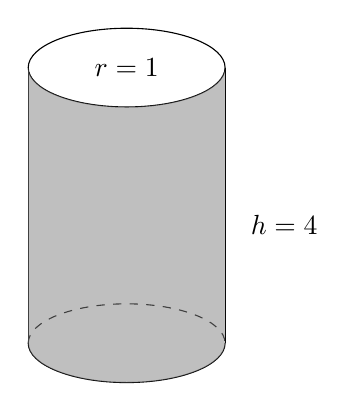
\begin{tikzpicture}
\draw (0,0) ellipse (1.25 and 0.5);
\draw (-1.25,0) -- (-1.25,-3.5);
\draw (-1.25,-3.5) arc (180:360:1.25 and 0.5);
\draw [dashed] (-1.25,-3.5) arc (180:360:1.25 and -0.5);
\draw (1.25,-3.5) -- (1.25,0);  
\fill [gray,opacity=0.5] (-1.25,0) -- (-1.25,-3.5) arc (180:360:1.25 and 0.5) -- (1.25,0) arc (0:180:1.25 and -0.5);
\draw (2,-2) node{$h = 4$};
\draw (0,0) node{$r = 1$};
\end{tikzpicture}
\end{align*}

El volumen del agua en función de la altura sigue el modelo $V_{(h)} = 4\pi h$. 

La tasa media del volumen entre los puntos $[2;2,5]$ es:

\begin{align*}
    V_m &= \frac{V_{(2,5)} - V_{(2)}}{2,5-2}\\
    V_m &= \frac{4\pi\frac{5}{2} - 4\pi 2}{\frac{5}{2}-2}\\
    V_m &= 4\pi
\end{align*}

Dados dos puntos cualesquiera, $a$ y $b$, llegamos a la siguiente expresión:

\begin{align*}
    V_m &= \frac{V_{(b)} - V_{(a)}}{b-a}\\
    V_m &= \frac{4\pi b - 4\pi a}{b-a}\\
    V_m &= \frac{4\pi \cancel{(b - a)}}{\cancel{b-a}}\\
    V_m &= 4\pi
\end{align*}

Con ello podemos concluir que, a diferencia de lo que ocurría en el modelo anterior, en este caso la pendiente permanece constante a lo largo de la función, por lo cual la velocidad media es mejor indicador del cambio en la función.
\subsection*{3}

Modelos de automóvil 1 y 2.

\begin{align*}
    D_1 &= t &
    D_2 &= \frac{t^2}{2}
\end{align*}

\subsubsection*{Parte A}

\textbf{a)} Representación gráfica de los dos modelos.

\begin{center}
\begin{tikzpicture}
\begin{axis}[
    axis lines = left,
    xlabel = \(t\),
    ylabel = {\(D(t)\)},
    clip = false,
]
% D_1
\addplot [
    domain=0:10, 
    samples=200, 
    color=blue,
]
{x};
\addlegendentry{\(D_1=t\)}

% D_2
\addplot[
    domain=0:10,
    samples=200,
    color=red,
]
{x*x/2};
\addlegendentry{\(D_2=\frac{t^2}{2}\)}
\end{axis}
\end{tikzpicture}
\end{center}

\textbf{b)} Kilómetros recorridos al cabo de 1, 2 y 3 minutos.

\begin{center}
\begin{tabular}{ c c c }
	t	&	$D_1$  &   $D_2$  \\
	\hline \\
	1	&	1     &   $1/2$\\	
	2	&	2     &   2\\	
	3	&	3     &   $9/2$\\
    \hline
\end{tabular}
\end{center}

\textbf{c)} Velocidad media en intervalos [0, 1], [0, 2], [0, 3] y [1, 2].

\begin{center}
\begin{tabular}{ c c c }
	Intervalo	&	$D_1$  &   $D_2$ \\
	\hline \\
	$[0, 1]$    &	 1     &   $1/2$ \\	
	$[0, 2]$    &	 1     &   1     \\	
	$[0, 3]$    &	 1     &   $3/2$ \\
    $[1, 2]$    &    1     &   $3/2$ \\
    \hline
\end{tabular}
\end{center}

\textbf{Conclusiones.} Si observamos la velocidad media del modelo 1, rápidamente notamos que esta es constante a lo largo de la trayectoria. Esto es lo esperable de un modelo lineal. Al ser constante la pendiente, es esperable que el cambio en la misma, cualquiera sea el punto que se tome, permanezca constante, como se ha observado en el modelo anterior.

En lo que respecta al modelo 2, la situación es diferente. Nos encontramos ahora frente a un modelo cuadrático, por lo cual el cálculo de la velocidad media cambia según el período de tiempo considerado, siendo superior a medida que pasa el tiempo. 

Ello llevaría a concluir que uno de los automóviles se desplaza de manera uniforme, mientras el otro lo hace de manera uniformemente variada.

\vspace{10pt}

\textbf{d)} Para calcular la velocidad en los minutos 1 y 2 recurrimos a la derivada de cada una de las funciones:

\begin{align*}
    D_1' &= 1 &
    D_2' &= t
\end{align*}

\begin{center}
\begin{tabular}{ c c c }
	t	&	$D'_1$  &   $D'_2$  \\
	\hline \\
	1	&	1     &   1\\	
	2	&	1     &   2\\
    \hline
\end{tabular}
\end{center}

\textbf{e)} Las tangentes a la distancia recorrida por el automóvil 2, en los puntos 1 y 2, son las siguientes:

\begin{center}
\begin{tikzpicture}
\begin{axis}[
    axis lines = left,
    xlabel = \(t\),
    ylabel = {\(D(t)\)},
    clip = false,
]
% D'_2 en 1
\addplot [
    domain=0:10, 
    samples=200, 
    color=purple,
]
{x-0.5};
\addlegendentry{\(D'_{2(1)}=t-\frac{1}{2}\)}

% D'_2 en 1
\addplot [
    domain=0:10, 
    samples=200, 
    color=cyan,
]
{2*x-2};
\addlegendentry{\(D'_{2(2)}=2t-2\)}

% D_2
\addplot[
    domain=0:10,
    samples=200,
    color=orange,
]
{x*x/2};
\addlegendentry{\(D_2=\frac{t^2}{2}\)}
\end{axis}
\end{tikzpicture}
\end{center}

Las expresiones de las rectas tangentes se obtienen recurriendo a la notación punto-pendiente ($y-y_0 = m(x-x_0)$), despejando la $y$.

\vspace{10pt}

\textbf{f)} Como se desprende tanto de la tabla como de la representación gráfica, la velocidad del automóvil 1 es constante, mientras la del automóvil 2 se incrementa a medida que pasa el tiempo.


\subsubsection*{Parte B}

\begin{center}
\begin{tikzpicture}
\begin{axis}[
    axis lines = left,
    xlabel = \(t\),
    ylabel = {\(D(t)\)},
    clip = false,
]

% D_2
\addplot[
    domain=0:3,
    samples=200,
    color=cyan,
]
{x*x/2};
\addlegendentry{\(D_2=\frac{t^2}{2}\)}

% Derivada que pasa por 2
\addplot[
    domain=1:3,
    samples=200,
    color=orange,
]
{2*x-2};
\addlegendentry{\(D'_2=2t-2\)}

\node[label={270:{(2,2)}},circle,fill,inner sep=2pt] at (axis cs:2,2) {};

\end{axis}
\end{tikzpicture}
\end{center}

Para obtener la función que describe a la recta tangente a la función en el punto $(2, 2)$ expresamos este punto en la notación punto-pendiente, incluyendo como pendiente al valor devuelto por la derivada de $D_2$, que en ese punto es 2. Entonces:

\begin{align*}
    y-2 &= 2(x-2)\\
    y &= 2x - 4 + 2\\
    y &= 2x - 2
\end{align*}

Por otra parte, para obtener la función que describe la recta secante correspondiente al intervalo $[1,5; 2]$, calculamos en primer lugar su pendiente:

\begin{align*}
    m &= \frac{D_{2(2)} - D_{2(1,5)}}{2 - 1,5}\\
    m &= \frac{2 - 9/8}{2 - 1,5}\\
    m &= \frac{7}{4}
\end{align*}

Con la expresión de la pendiente, tomamos uno de los puntos por el cual deseamos que cruce, en este caso puede ser $(2, 2)$, y planteamos la función en notación punto-pendiente:

\begin{align*}
    y-2 &= \frac{7}{4}(x-2)\\
    y &= \frac{7}{4}x - \frac{7}{2} + 2\\
    y &= \frac{7}{4}x - \frac{3}{2}
\end{align*}

Con la expresión $y = \frac{7}{4}x - \frac{3}{2}$, podemos representar la secante.

\begin{center}
\begin{tikzpicture}
\begin{axis}[
    axis lines = left,
    xlabel = \(t\),
    ylabel = {\(D(t)\)},
    clip = false,
]

% D_2
\addplot[
    domain=1:3,
    samples=200,
    color=cyan,
]
{x*x/2};
\addlegendentry{\(D_2=\frac{t^2}{2}\)}

% Secante que pasa por 2
\addplot[
    domain=1.5:2,
    samples=200,
    color=magenta,
]
{7/4*x-3/2};
\addlegendentry{\(S=\frac{7}{4}t - \frac{3}{2}\)}

\node[label={270:{(2,2)}},circle,fill,inner sep=2pt] at (axis cs:2,2) {};
\node[label={270:{(1,5,9/8)}},circle,fill,inner sep=2pt] at (axis cs:1.5,1.125) {};
\end{axis}
\end{tikzpicture}
\end{center}

\begin{center}
\begin{tabular}{ c c c c c c c c c c c c }
    t & 1,5 & 1,9 & 1,99 & 1,999 & 1,9999 & 2 & 2,0001 & 2,001 & 2,01 & 2,1 & 2,5\\
	\hline \\
    $g_{(t)} = \frac{t^2}{2}$ & 1.125 & 1.805 & 1.98 & 1.998 & 1.9998 & 2 & 2.0002 & 2.002 & 2.02 & 2.205 & 3.125 \\
    \vspace{10pt} \\
    $\frac{g_(t) - g_(2)}{t - 2}$ & 1.75 & 1.95 & 2 & 2 & 2 & 2 & 2 & 2 & 2 & 2.05 & 2.25\\
    \vspace{10pt} \\
    \hline
\end{tabular}
\end{center}

Como puede observarse tanto en las gráficas como en la tabla construida, a medida que los extremos de la recta secante se aproximan, el valor de su pendiente tiende al valor de la derivada en dicho punto.
\section*{Actividad 2}

Para aproximarnos al problema de la princesa Dido desde la optimización, podemos imaginar una elipse, cuyos semiejes denominaremos $a$ y $b$.

\begin{center}
    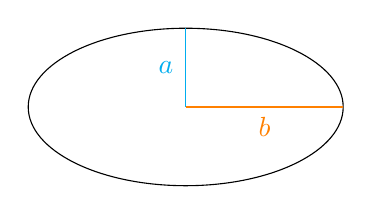
\begin{tikzpicture}
        \draw (0,0) ellipse (2cm and 1cm);
        \draw[-, cyan] (0,0) -- (0,1); % línea a
        \draw[cyan] (-0.25,0.5) node{$a$}; % label a
        \draw[-, orange] (0,0) -- (2,0); % línea b
        \draw[orange] (1,-0.25) node{$b$}; % label b
    \end{tikzpicture}
\end{center}

Podemos plantear dos ecuaciones, una para su área:

\begin{align*}
    A &= \pi ab
\end{align*}

Y otra para su perímetro:

\begin{align*}
    P &= \pi (a + b)
\end{align*}

En nuestro caso, el perímetro funciona como una restricción, a partir de la cual podemos despejar $a$, para expresar el área del elipse en función de $b$:

\begin{align*}
    \pi (a + b) &= 100\\
    a &= \frac{100}{\pi} - b
\end{align*}

Expresamos el área en función de $b$:

\begin{align*}
    A &= \pi b (\frac{100}{\pi} - b)\\
    A &= 100b - \pi b^2
\end{align*}

Derivamos esta función:

\begin{align*}
    \frac{dA}{dx} &= 100 - 2 \pi b
\end{align*}

E igualamos a 0, para determinar el punto máximo de la función del área:

\begin{align*}
    100 - 2 \pi b &= 0\\
    b &= \frac{-100}{-2 \pi}\\
    b &= \frac{50}{\pi}
\end{align*}

De ahí determinamos que $a$ es: 

\begin{align*}
    a &= \frac{100}{\pi} - \frac{50}{\pi}\\
    a &= \frac{50}{\pi}\\
    a &= b
\end{align*}

La elipse cuyos semiejes son iguales, en este caso $a$ y $b$, es el círculo. El círculo sería entonces la figura que maximizaría el área.

\section*{Unidad 5: Integrales y aplicaciones}

\subsection*{Métodos de integración}

\begin{figure}
    \centering
    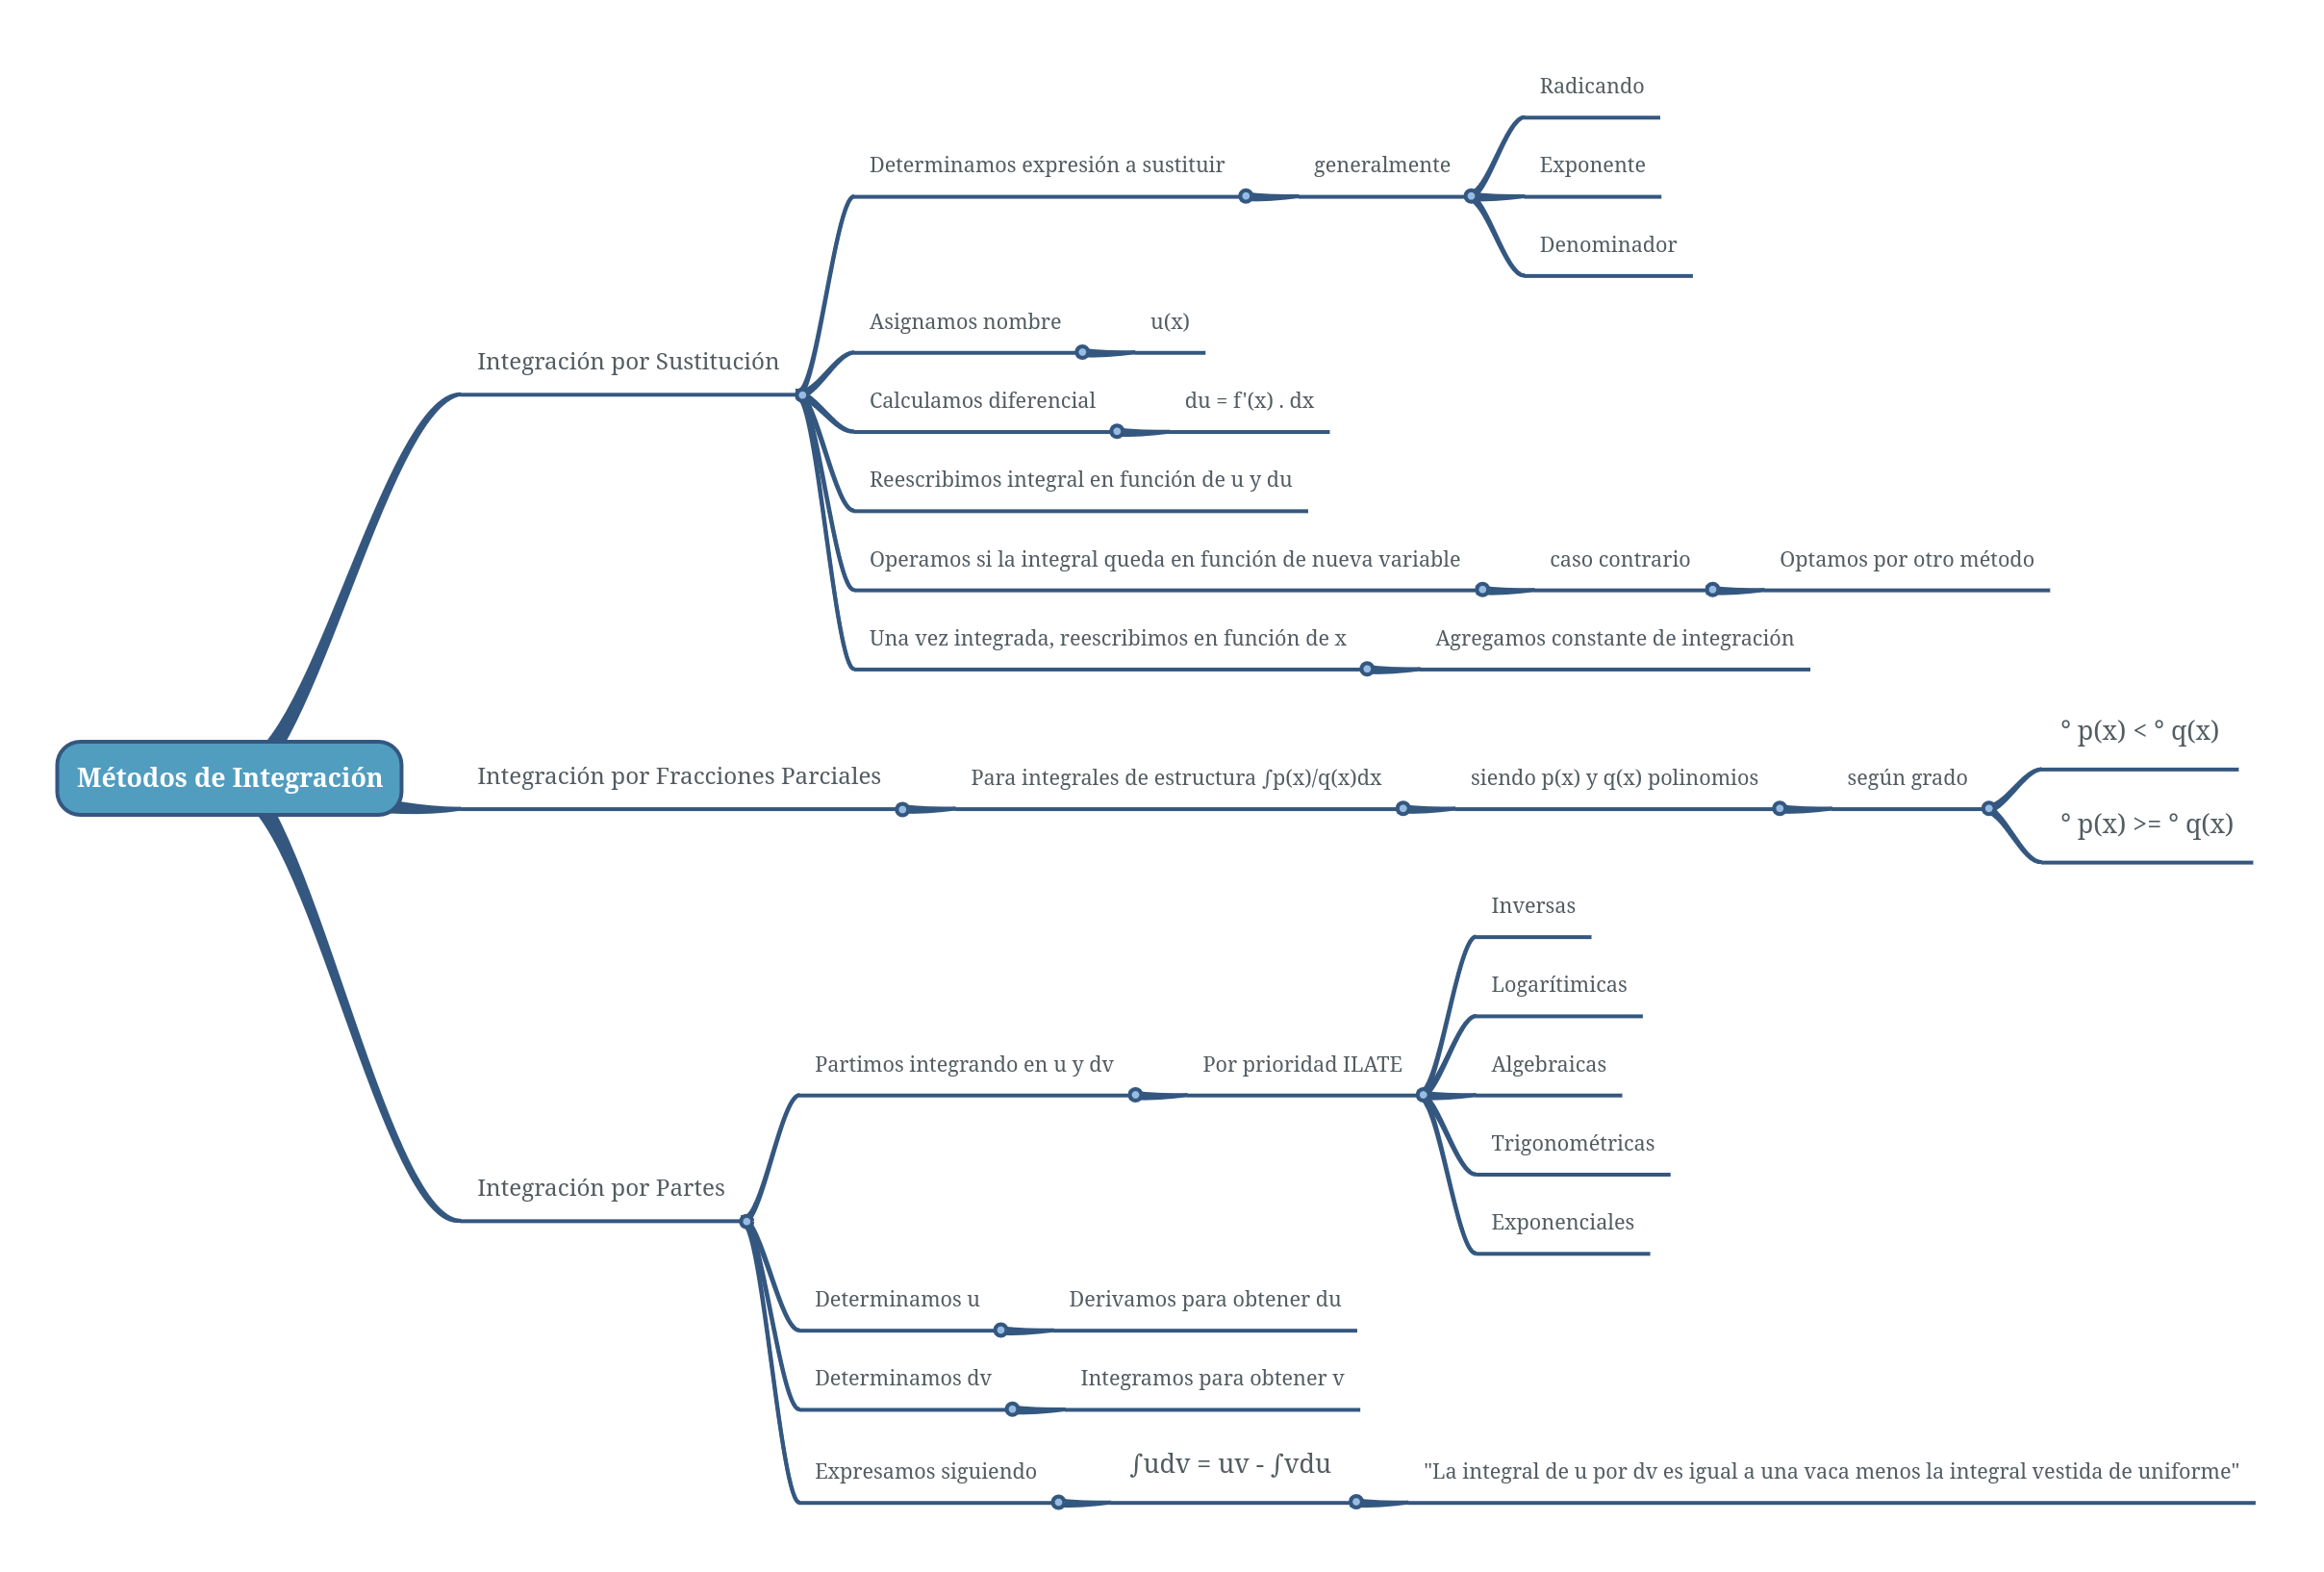
\includegraphics[width=20cm, angle=270]{img/metodos integracion.png}
    \caption{Métodos de Integración}
    \label{fig:metodos-integracion}
\end{figure}

\begin{figure}
    \centering
    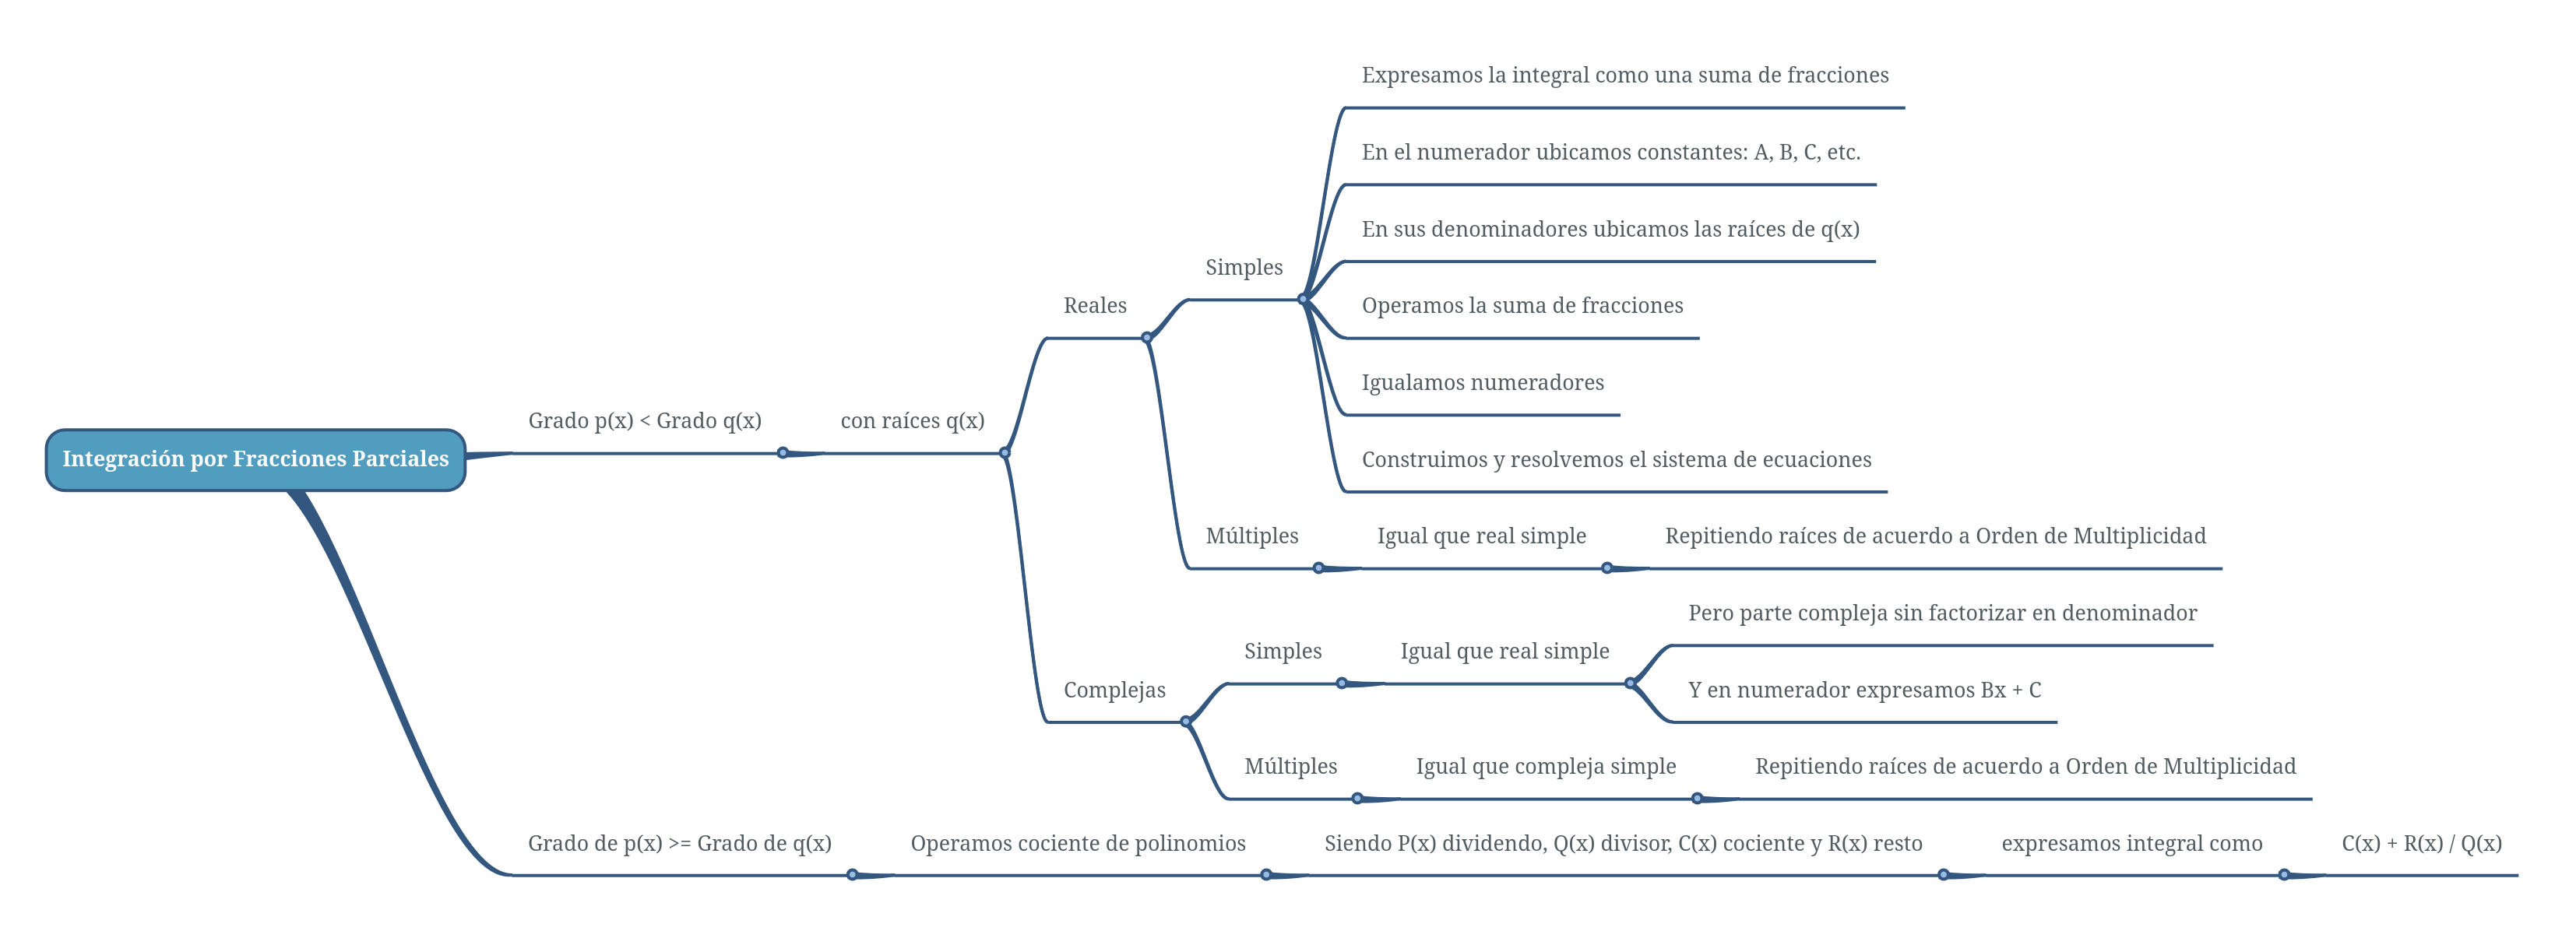
\includegraphics[width=22cm, angle=270]{img/integracion por fracciones parciales.png}
    \caption{Integración por fracciones parciales}
    \label{fig:integracion-fracciones-parciales}
\end{figure}

\subsection*{Parte B}

\subsection*{Actividad 1}

El problema pide calcular el desplazamiento y la distancia recorrida por un drone, dada una función de su velocidad, medida en $\frac{m}{s}$. La velocidad del drone viene definida por la función $V_{(t)} = t^2 - t - 6$. 

\begin{center}
\begin{tikzpicture}
\begin{axis}[
    axis lines = middle,
    xlabel = \(t\),
    ylabel = {\(V(t)\)},
    clip = false,
]
% V_t
\addplot [
    domain=0:4, 
    samples=200, 
    color=cyan,
]
{x*x-x-6};
\addlegendentry{\(V_{(t)} = t^2 - t - 6\)}

\end{axis}
\end{tikzpicture}
\end{center}

Si operamos la integral de esta función -que, al tratarse de un polinomio, se puede hacer de manera directa- obtenemos la función $d_{(t)} = \frac{t^3}{3} - \frac{t^2}{2} - 6t + C$. Notar que la primitiva de la función expresa el área bajo la curva, por lo que estaría expresada en $m$. Sería entonces una función que devolvería la distancia recorrida por el Drone.

Se nos pide considerar el desplazamiento dentro del intervalo $[1, 4]$. Sin embargo, en el intervalo $[1, 3]$ la integral sería negativa. Ello nos invita a pensar que el drone, en ese período, se desplazó en un sentido, cambiando dicho sentido en $(3, 4]$. 

Entonces, podríamos pensar que el desplazamiento final del drone implicaría restar las distancias recorridas. Por su parte, obtener la distancia recorrida total implicaría sumar el módulo de ambos desplazamientos, con independencia del sentido en que el drone se haya desplazado.

Operamos la integral definida para cada uno de estos intervalos.

\begin{align*}
    \int_{1}^{3} t^2 - t - 6 \,dx &= \frac{t^3}{3} - \frac{t^2}{2} - 6t \Big|_1^3\\
    \frac{3^3}{3} - \frac{3^2}{2} - 6 \cdot 3 &- \left( \frac{1^3}{3} - \frac{1^2}{2} - 6 \cdot 1 \right)\\
    - \frac{22}{3}
\end{align*}

\begin{align*}
    \int_{3}^{4} t^2 - t - 6 \,dx &= \frac{t^3}{3} - \frac{t^2}{2} - 6t \Big|_3^4\\
    \frac{4^3}{3} - \frac{4^2}{2} - 6 \cdot 4 &- \left( \frac{3^3}{3} - \frac{3^2}{2} - 6 \cdot 3 \right)\\
    \frac{17}{6}
\end{align*}

Entonces, el desplazamiento del drone vendría dado por la expresión $\frac{17}{6} - \frac{22}{3}$, siendo $- \frac{9}{2}$. Por su parte, el recorrido total sería $|\frac{17}{6}| + |\frac{22}{3}|$, siendo $\frac{61}{6}$ el recorrido total del drone.
\end{document}
